%
\chapter{Marco Te\'orico}

Se definen las tecnolog\'as y conceptos te\'oricos que se utilizar\'an en el desarrollo del presente trabajo.


\section{Twitter}
\setcounter{equation}{0}

Es una plataforma de servicio de microblogging que permite el envi\'o de mensajes de texto en un tamaño m\'aximo de 280 caracteres denominados tweets, los usuarios pueden subscribirse a los tweets de otros usuarios y hacerles seguimientos, esta acci\'on es conocida como seguidores o followers. Por defecto los mensajes son p\'ublicos y pueden contener la zona geogr\'afica de la persona que ha enviado el tweet.\\

A continuaci\'on se muestra la estructura de un tweet:

\begin{table}[H]

\begin{center}
\begin{tabular}{ |p{2cm}|p{2cm}|p{6cm}| }
\hline
\rowcolor{gray!40}  \textbf{Atributo}         & \textbf{Tipo}      & \textbf{Descripci\'on}   \\  \hline
 created\_at   & String  & Hora de creaci\'on.        \\   \hline
 Id                  & Int64   & Identificador del tweet.  \\   \hline
 text                & String  & El mensaje de texto.  \\   \hline
 source           & String  & Usado para postear un texto en HTML.  \\   \hline
 user               & User    & Usuario que envia el mensaje de texto.  \\   \hline
 Coordinates   & Coordinates   & Coordenadas de la localizaci\'on geogr\'afica.  \\   \hline
 Retweeted     & Boolean   & Verifica si el mensaje ha sido reenviado.  \\   \hline
 Lang               & String   & Idioma del mensaje.  \\   \hline
\end{tabular}
\caption{Estructura de un tweet obtenido de la Empresa Twitter}

\end{center}
\end{table}
		
	 	
		
		
		



\section{Data Mining}

El Data Mining es un campo de la estad\'istica y las ciencias de la computaci\'on relacionado con el proceso de descubrir patrones en grandes vol\'umenes de conjuntos de datos. Utiliza m\'etodos de inteligencia artificial, aprendizaje autom\'atico, estad\'istica y sistemas de bases de datos \\	

La forma para aplicar Data Mining se basa en las siguientes etapas:

\begin{itemize}
\item Comprensión del Negocio.
\item Comprensión de los Datos.
\item Preparación de los datos.
\item Modelado
\item Evaluación 
\item Desarrollo
\end{itemize}

\section{Text Mining}

Es el an\'alisis de informaci\'on no estructurada, la cual se puede encontrar en redes sociales, para tal fin se emplea t\'ecnicas de ling\"uística, modelamientos estad\'isticos y t\'ecnicas de aprendizaje para descubrir conocimientos que no existen explícitamente en ning\'un texto de la colecci\'on, pero que surgen al relacionar el contenido de muchos de ellos. \\

Se suelen aplicar a encuestas de opini\'on, encuestas de satisfacci\'on, libros de reclamaci\'on, etc. \\

La forma para aplicar Text Mining se basa en las siguientes etapas:

\begin{itemize}
\item Preparar texto para el análisis
\item Extraer conceptos
\item Aplicar el análisis de enlace de texto
\item Construir categorías
\item Desplegar modelos predictivos
\end{itemize}

Los beneficios del uso del text mining es que nos permite identificar hechos o datos puntuales a partir del texto de los documentos, agrup\'andolo en clustering e igualmente determinar el tema o temas tratados en los documentos mediante la categorizaci\'on autom\'atica de los textos y crear redes de conceptos.
		
\begin{itemize}
\item El text mining  se puede aplicar en:
\item Resumen autom\'atico de textos
\item Detecci\'on de fraudes
\item Tendencial electorales
\item An\'alisis de Sentimiento
\item Clasificaci\'on de textos.
\end{itemize}

\section{An\'alisis de Sentimiento}

Es el uso del procesamiento del lenguaje natural, an\'alisis de texto y ling\"aística computacional para identificar y extraer informaci\'on subjetiva de los recursos. Desde el punto de vista de la minería de textos, el an\'alisis de sentimientos es una tarea de clasificaci\'on masiva de documentos de manera autom\'atica, en funci\'on de la connotaci\'on positiva o negativa del lenguaje ocupado en el documento. Es importante mencionar que estos tratamientos generalmente "se basan en relaciones estad\'isticas y de asociaci\'on, no en an\'alisis ling\"uístico".

\subsection{T\'ecnicas de An\'alisis de Sentimiento}

Seg\'un Medhat, las principales t\'ecnicas de an\'alisis de sentimiento se dividen en dos grandes grupos: las que se basan en aprendizaje autom\'atico (machine learning approach) y las que se basan en diccionarios (lexicon-based approach). \\

La siguiente figura muestra las 2 técnicas:\\

\begin{figure}[H]
\centering
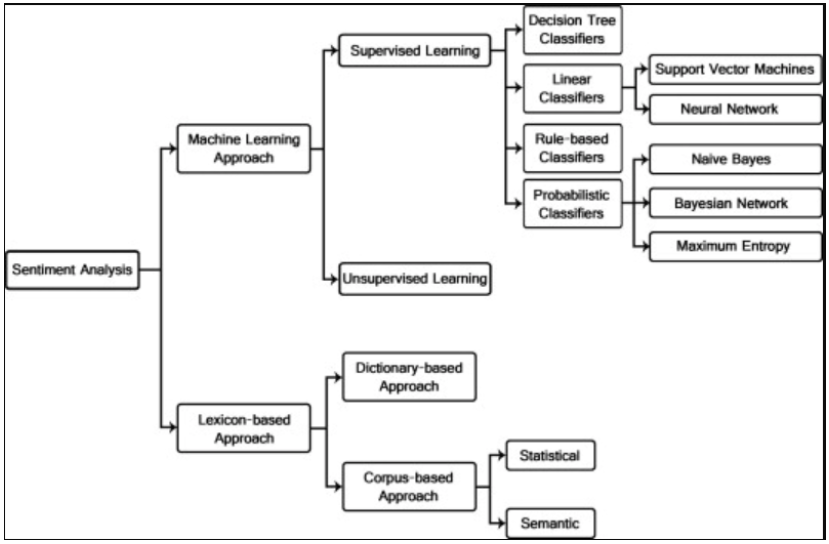
\includegraphics[scale=0.4]{chapters/img/Ch05_Medhat.PNG}
\caption{Técnicas de An\'alisis de Sentimiento seg\'un Medat}
\end{figure}

Una vez mostrado los m\'etodos de an\'alisis, en la presente investigación se usará la estrategia de los algoritmos de aprendizaje automático que tiene relación con el campo de la informática y más en concreto, de la inteligencia artificial.

 El procesamiento de datos es a trav\'es del aprendizaje para tal fin se extrae patrones de comportamiento a partir de las entradas recibidas, y en base a dicha informaci\'on aprendida o asimilada, realice la evaluaci\'on de nuevas entradas. Los algoritmos internos que constituyen la base de este aprendizaje tienen un fuerte componente estad\'istico y algebraico, con la consiguiente capacidad de c\'alculo.



\cleardoublepage